% ==============================================================================
% SLIDE 2: MOTIVATION
% ==============================================================================
\begin{frame}
	\frametitle{Motivation}
	\begin{itemize}
		\item Housing prices and rents are skyrocketing in many U.S.\ cities, including Chicago
		\begin{itemize}
			\item Limited housing supply in high demand areas is widely accepted as the key driver of these price increases
			\item Land use regulations and local control are often blamed for limiting supply
		\end{itemize}
		\item Most research focuses on formal institutions such as by-right zoning laws or planning commissions
		\begin{itemize}
			\item But regulatory uncertainty, permitting delays, and discretion are also key determinants of housing supply and are less studied
		\end{itemize}
		\item \textbf{Chicago}: Unique informal institution of \textit{aldermanic privilege}
		\begin{itemize}
			\item Offers a unique setting where de facto regulatory environment changes discretely at ward boundaries
		\end{itemize}
	\end{itemize}
\end{frame}

% ==============================================================================
% SLIDE 4: WHAT IS ALDERMANIC PRIVILEGE?
% ==============================================================================
\begin{frame}
	\frametitle{What is Aldermanic Privilege?}
	\begin{itemize}
		\item \textbf{Not written in any law} --- Chicago has no city charter
		\item An informal but extraordinarily powerful norm
		\item Core feature: \textbf{Deference}
		\begin{itemize}
			\item Other aldermen essentially never override a colleague's decision in their ward
			\item ``Very few things happen that aldermen don't want to happen.'' \mbox{\scriptsize \citep{zhang_boundaries_2011}}
			\item Encyclopedia of Chicago: ``little mayors'' ruling wards as ``fiefdoms''
		\end{itemize}
		\item \textbf{Chicago gives more power to local politicians than many other U.S.\ cities}: 
		\begin{itemize}
			\item Houston has no explicit zoning code and centralized development approvals
			\item Minneapolis has reduced councilmember discretion in recent years
			\item Both cities have seen below-median rent and home price growth compared to peer cities \cite{hembre_unpacking_2025,heckler_this_2026}
		\end{itemize}
	\end{itemize}
\end{frame}



% ==============================================================================
% SLIDE 3: NEWS HEADLINES (existing slide, kept)
% ==============================================================================
\begin{frame}
	\frametitle{Aldermanic Privilege is a Hotly Contested Issue in Chicago} 
    \begin{minipage}{0.5\textwidth}
        \begin{figure}
            \centering
            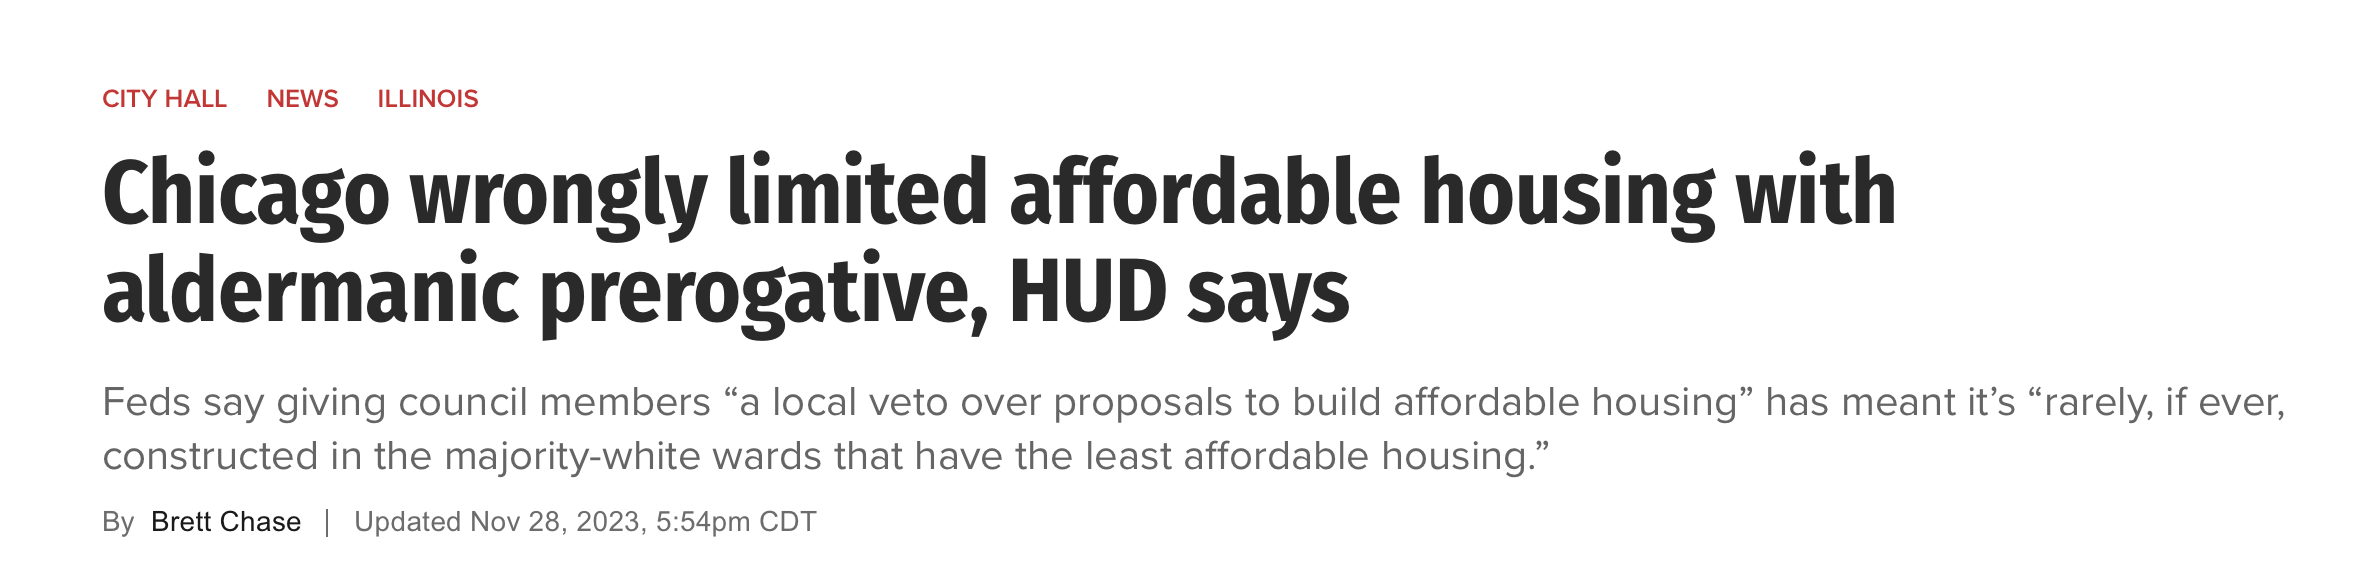
\includegraphics[width=\textwidth]{images/hud_report_headline.png}
		\end{figure}
		\begin{figure}
			\centering
			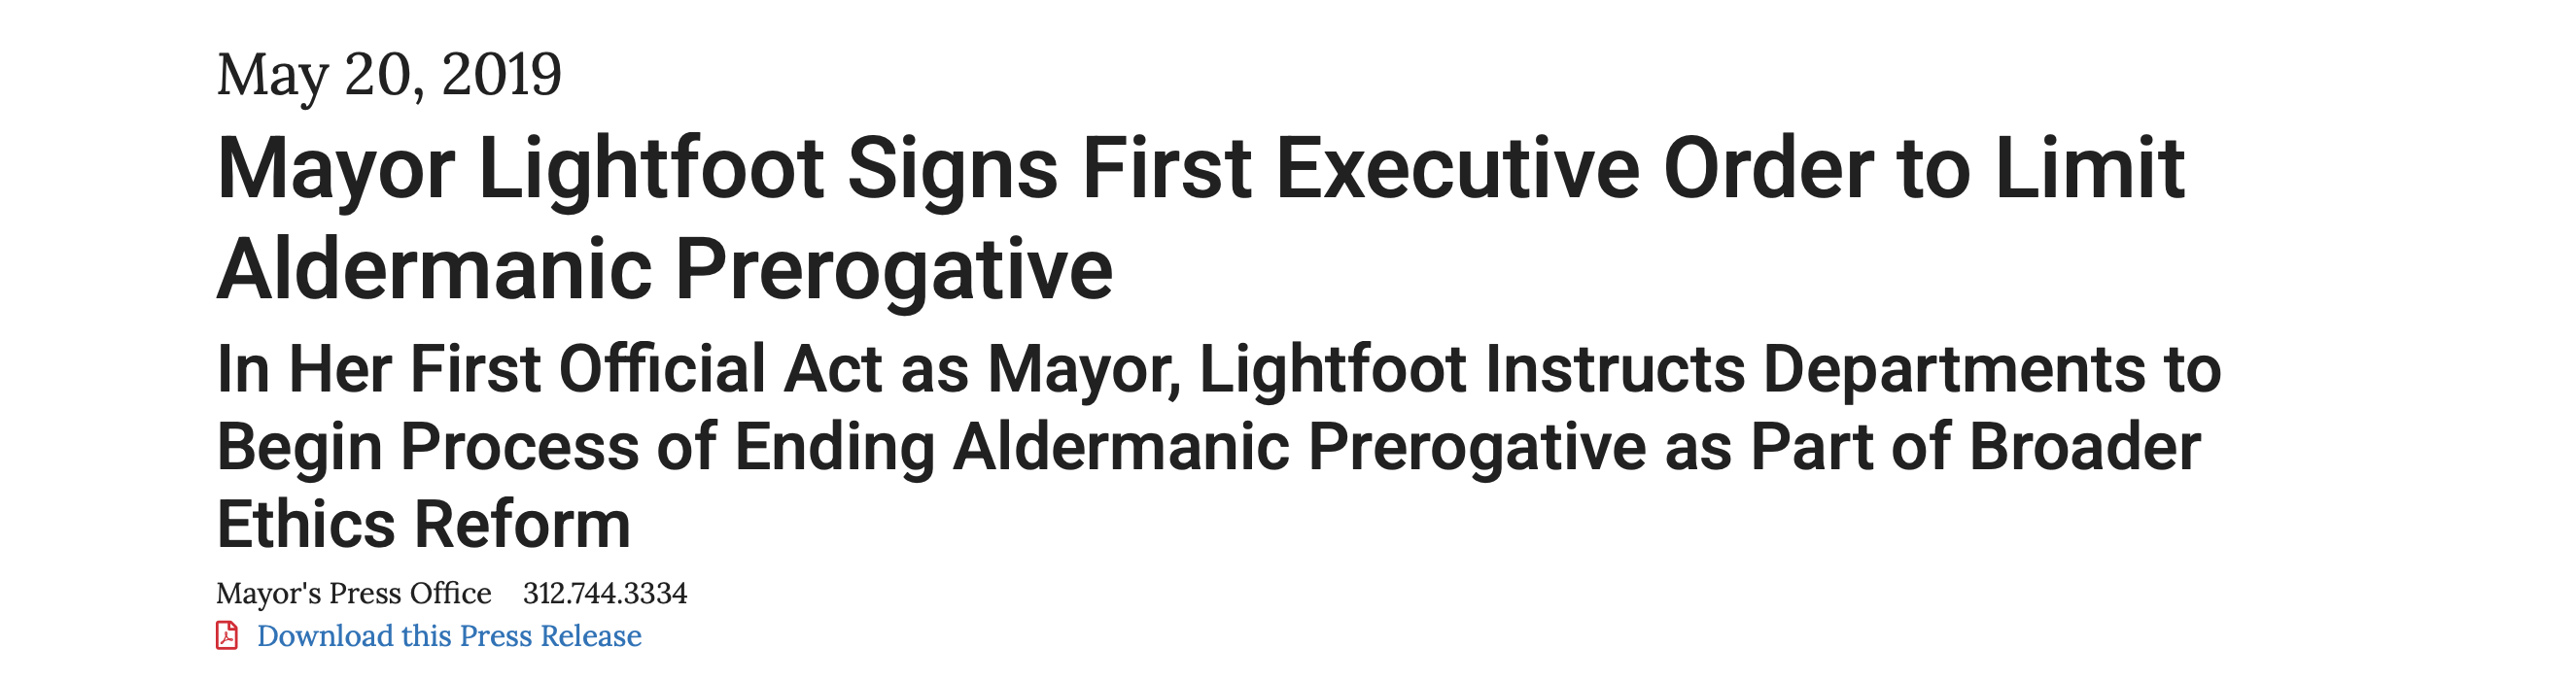
\includegraphics[width=\textwidth]{images/lightfoot_order.png}
		\end{figure}
		\begin{figure}
			\centering
			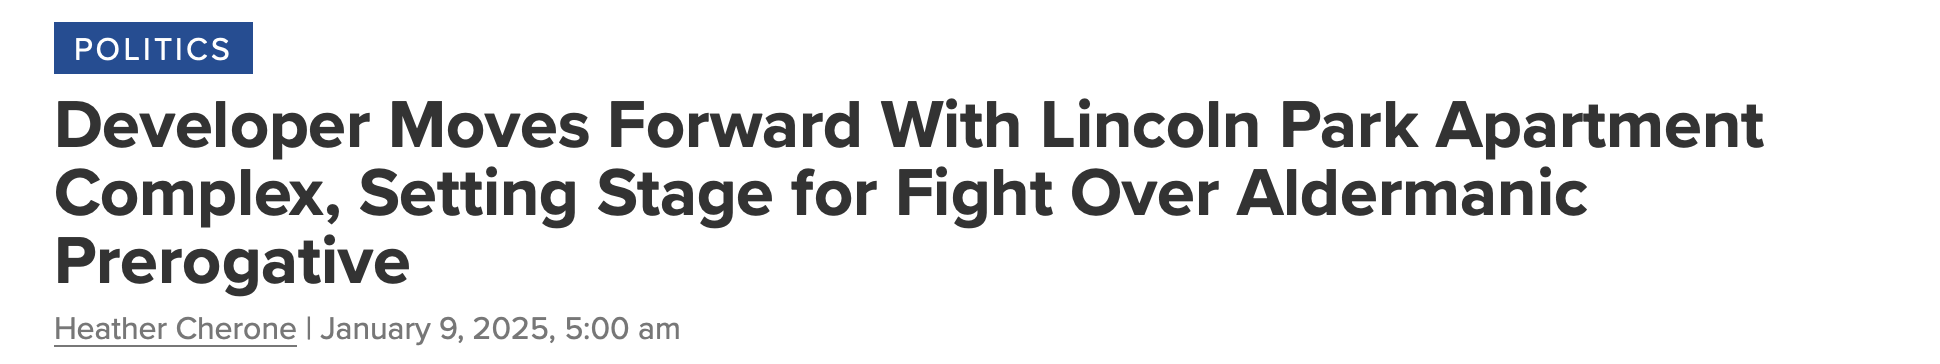
\includegraphics[width=\textwidth]{images/alderman_fight.png}
		\end{figure}
        \end{minipage}
        \hfill
        \begin{minipage}{0.48\textwidth}
        \begin{figure}
            \centering
            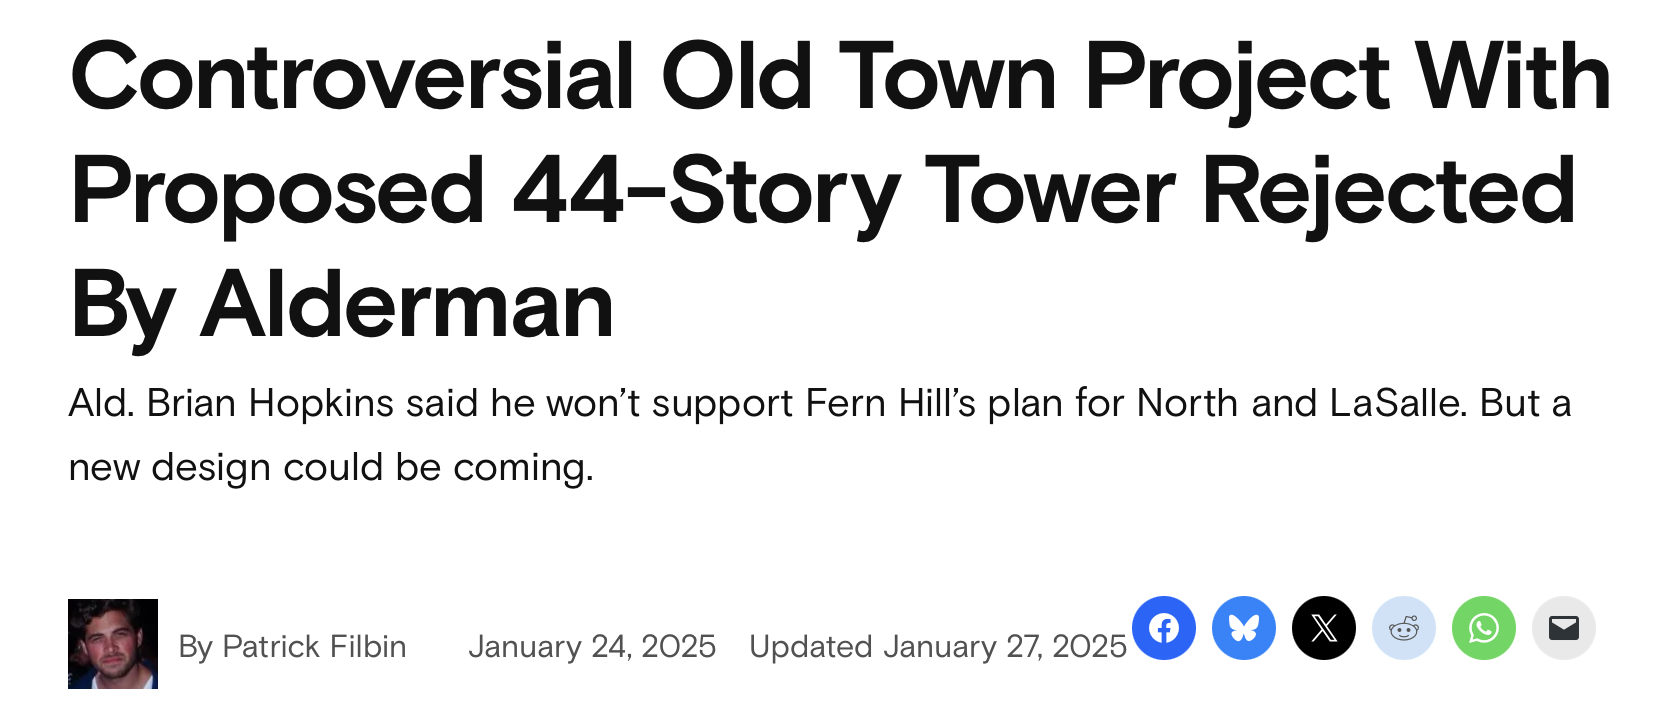
\includegraphics[width=\textwidth]{images/old_town_towers.png}
		\end{figure}
		\begin{figure}
			\centering
			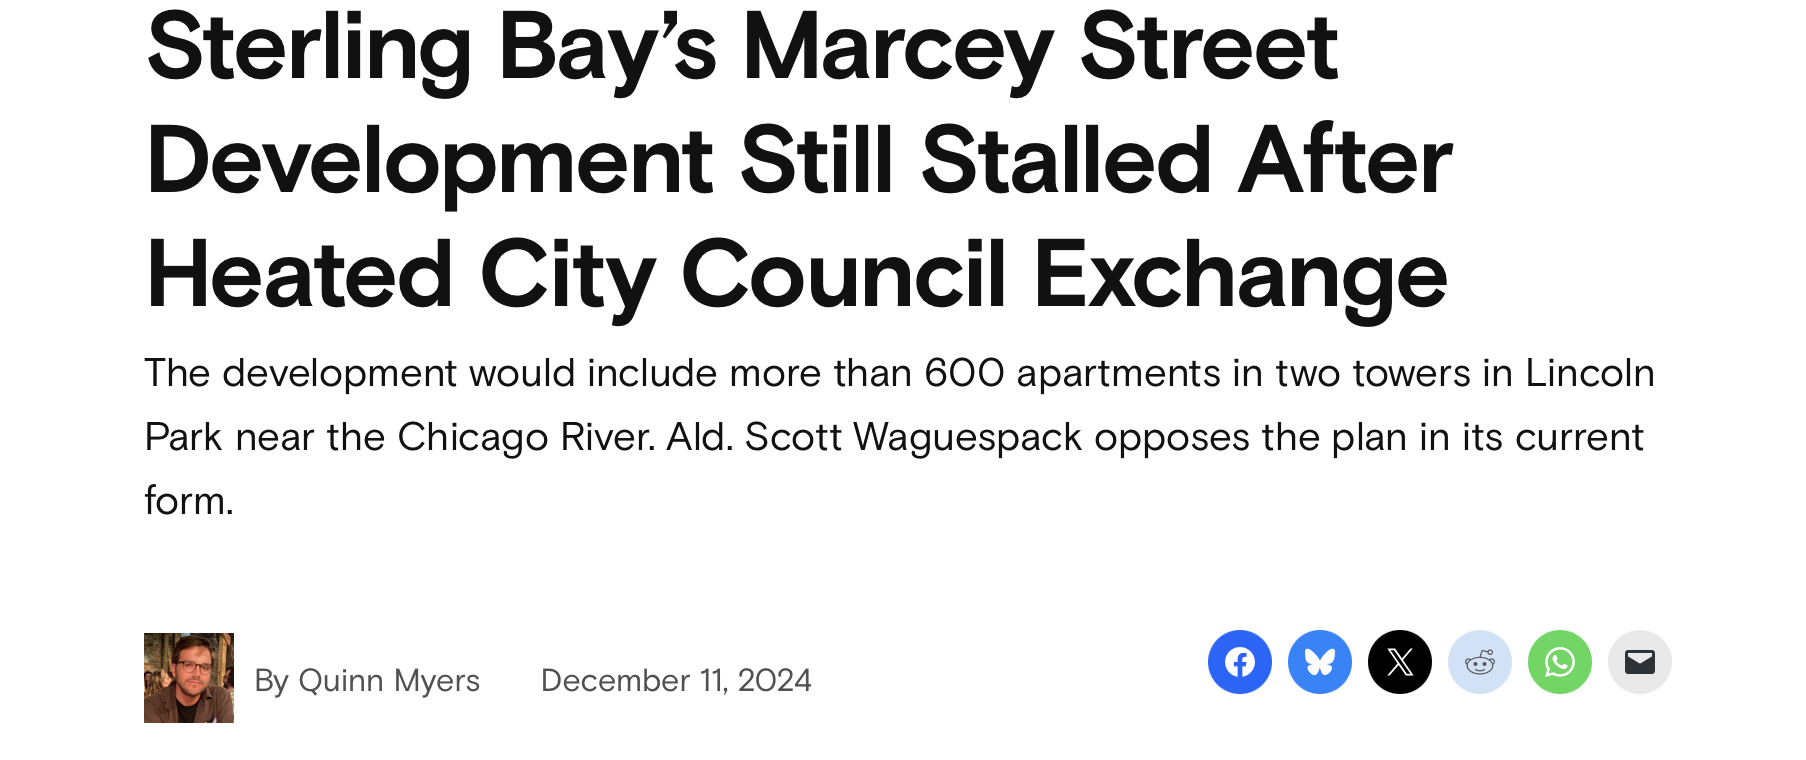
\includegraphics[width=\textwidth]{images/sterling_bay_fight.png}
        \end{figure}
        \end{minipage}
\end{frame}

% ==============================================================================
% SLIDE 5: HOW ZONING WORKS IN CHICAGO
% ==============================================================================
\begin{comment}
\begin{frame}
	\frametitle{How Zoning Works in Chicago}
	\textbf{Formal Process:}
	\begin{enumerate}
		\item Developer wants more density than as-of-right $\rightarrow$ requests rezone
		\item Application goes to Zoning Administrator $\rightarrow$ Dept.\ of Planning $\rightarrow$ Committee on Zoning $\rightarrow$ City Council vote
	\end{enumerate}
	
	\vspace{0.1em}
	\textbf{Informal Reality:}
	\begin{itemize}
		\item Alderman consulted at \textit{every} step (even though not formally required)
		\item Many aldermen have their own ward application forms
		\item Alderman says yes $\rightarrow$ passes unanimously
		\item Alderman says no $\rightarrow$ dead on arrival (colleagues defer, often no city council vote)
	\end{itemize}
	\textbf{Result:}
	\begin{itemize}
		\item De facto veto power creates a tremendous amount of uncertainty for developers
	\end{itemize}
\end{frame}
\end{comment}

% ==============================================================================
% SLIDE 6: THIS PAPER
% ==============================================================================
\begin{frame}
	\frametitle{This Paper}
	\textbf{Research Question}: Does the heterogeneity in regulatory uncertainty induced by aldermanic privilege reduce housing supply and raise prices?

	\vspace{0.5em}
	\textbf{Empirical strategy}: Segment-localized border design at ward boundaries
	\begin{itemize}
		\item Main density specification uses zoning-code + boundary-segment + year fixed effects (500 ft multifamily sample)
	\end{itemize}

	\vspace{0.3em}
	\textbf{Preview of Results}
	\begin{enumerate}
		\item More uncertain aldermen $\Rightarrow$ lower multifamily FAR and DUPAC near ward borders (about 7--10\% in border FE)
		\item $\sim$2\% higher rents on the more stringent side of the border 
		\item Effect appears to operate through reduced supply
	\end{enumerate}
\end{frame}
